% !TeX program = xelatex
% !TeX encoding = UTF-8
\documentclass{JXUSTmodeling}
\biaoti{论文题目待定}
\keyword{数学建模；优化模型；敏感性分析；Python}
\begin{document}
\begin{abstract}
  本文针对题目中的若干问题，建立了可复现、可解释并便于检验的数学模型。当前摘要为占位内容，待题目、数据、模型结果和最终图表确认后，由 Codex 按照中国大学生数学建模竞赛优秀论文风格重写。


\end{abstract}
\section{问题的提出}\label{sec:1}
\subsection{问题的背景}\label{sub:1.1}

待导入题目背景。

\subsection{已知的条件}\label{sub:1.2}

待整理题目给定条件、数据附件和限制条件。

\subsection{问题的提出}\label{sub:1.3}

本文需要解决的问题可概括如下：

\begin{enumerate}
  \item 问题一：待填写；
  \item 问题二：待填写；
  \item 问题三：待填写；
  \item 问题四：如题目包含则填写；
  \item 问题五：如题目包含则填写。
\end{enumerate}


\section{问题的分析}\label{sec:2}
\subsection{问题的整体分析}\label{sub:2.1}

待 Codex 根据题面和数据补充整体建模路线。

\subsection{问题一的分析}\label{sub:2.2}

待补充。

\subsection{问题二的分析}\label{sub:2.3}

待补充。

\subsection{问题三的分析}\label{sub:2.4}

待补充。

\subsection{问题四的分析}\label{sub:2.5}

如题目包含问题四，则在此补充。

\subsection{问题五的分析}\label{sub:2.6}

如题目包含问题五，则在此补充。


\section{模型的假设}\label{sec:3}
为简化问题并保证模型可求解，本文将在题面和数据检查完成后给出模型假设。每条假设均需说明其合理性和可能带来的影响。

\begin{enumerate}
  \item 假设一：待填写；
  \item 假设二：待填写；
  \item 假设三：待填写。
\end{enumerate}



\section{符号说明}\label{sec:4}
\begin{table}[htbp]
  \centering
  \caption{主要符号说明}
  \begin{tabularx}{\textwidth}{cYc}
    \toprule
    符号 & 含义 & 单位 \\
    \midrule
    $x$ & 待定义变量 & - \\
    \bottomrule
  \end{tabularx}
\end{table}



\section{模型的建立与求解}\label{sec:5}
\subsection{问题一模型的建立与求解}\label{sub:5.1}

问题一要求分析男胎胎儿的 Y 染色体浓度与孕周、孕妇 BMI 等因素之间的关系。由于同一孕妇存在多次检测记录，若直接随机划分训练集和测试集，容易把同一孕妇的个体差异泄漏到验证集中。因此本文在问题一中采用按孕妇代码分组的交叉验证，并在非线性关系刻画上使用样条岭回归模型。

\subsubsection{数据预处理与变量定义}

记第 $i$ 名孕妇第 $j$ 次检测的孕周为 $t_{ij}$，孕妇 BMI 为 $b_i$，男胎 Y 染色体浓度为 $y_{ij}$，测序质量控制变量向量为 $\boldsymbol q_{ij}$。根据题目中男胎检测数据的可解释范围，本文保留孕周在 $10$ 至 $25$ 周内、Y 染色体浓度为正且核心字段完整的样本。清洗后样本量为 1068 条，涉及 267 名孕妇；孕周范围为 11.0–24.9 周，BMI 范围为 20.7–46.9。

\subsubsection{样条岭回归模型}

考虑孕周和 BMI 与 Y 染色体浓度之间可能存在非线性关系，本文采用 B 样条基函数分别展开孕周和 BMI，并加入二者的交互项。模型形式为
\[
  y_{ij}=\beta_0+f_1(t_{ij})+f_2(b_i)+f_3(t_{ij},b_i)+\boldsymbol{\gamma}^{\mathrm T}\boldsymbol q_{ij}+\varepsilon_{ij},
\]
其中 $f_1(\cdot)$ 和 $f_2(\cdot)$ 分别表示孕周与 BMI 的非线性边际效应，$f_3(\cdot,\cdot)$ 表示二者的交互影响，$\varepsilon_{ij}$ 为随机误差项。为降低样条展开后多重共线性对估计稳定性的影响，模型采用岭回归惩罚：
\[
  \min_{\boldsymbol\theta}\sum_{i,j}\left(y_{ij}-\hat y_{ij}\right)^2+\alpha\|\boldsymbol\theta\|_2^2 .
\]

样条阶数在 $3$ 至 $6$ 之间比较，外层采用 5 折 GroupKFold，内层按孕妇分组选择惩罚参数 $\alpha$。最终选择样条阶数 3、节点数 5、惩罚参数 $\alpha=88.5867$ 的模型。建模流程如 \ref{fig:q1_flow} 所示。

\begin{figure}[htbp]
  \centering
  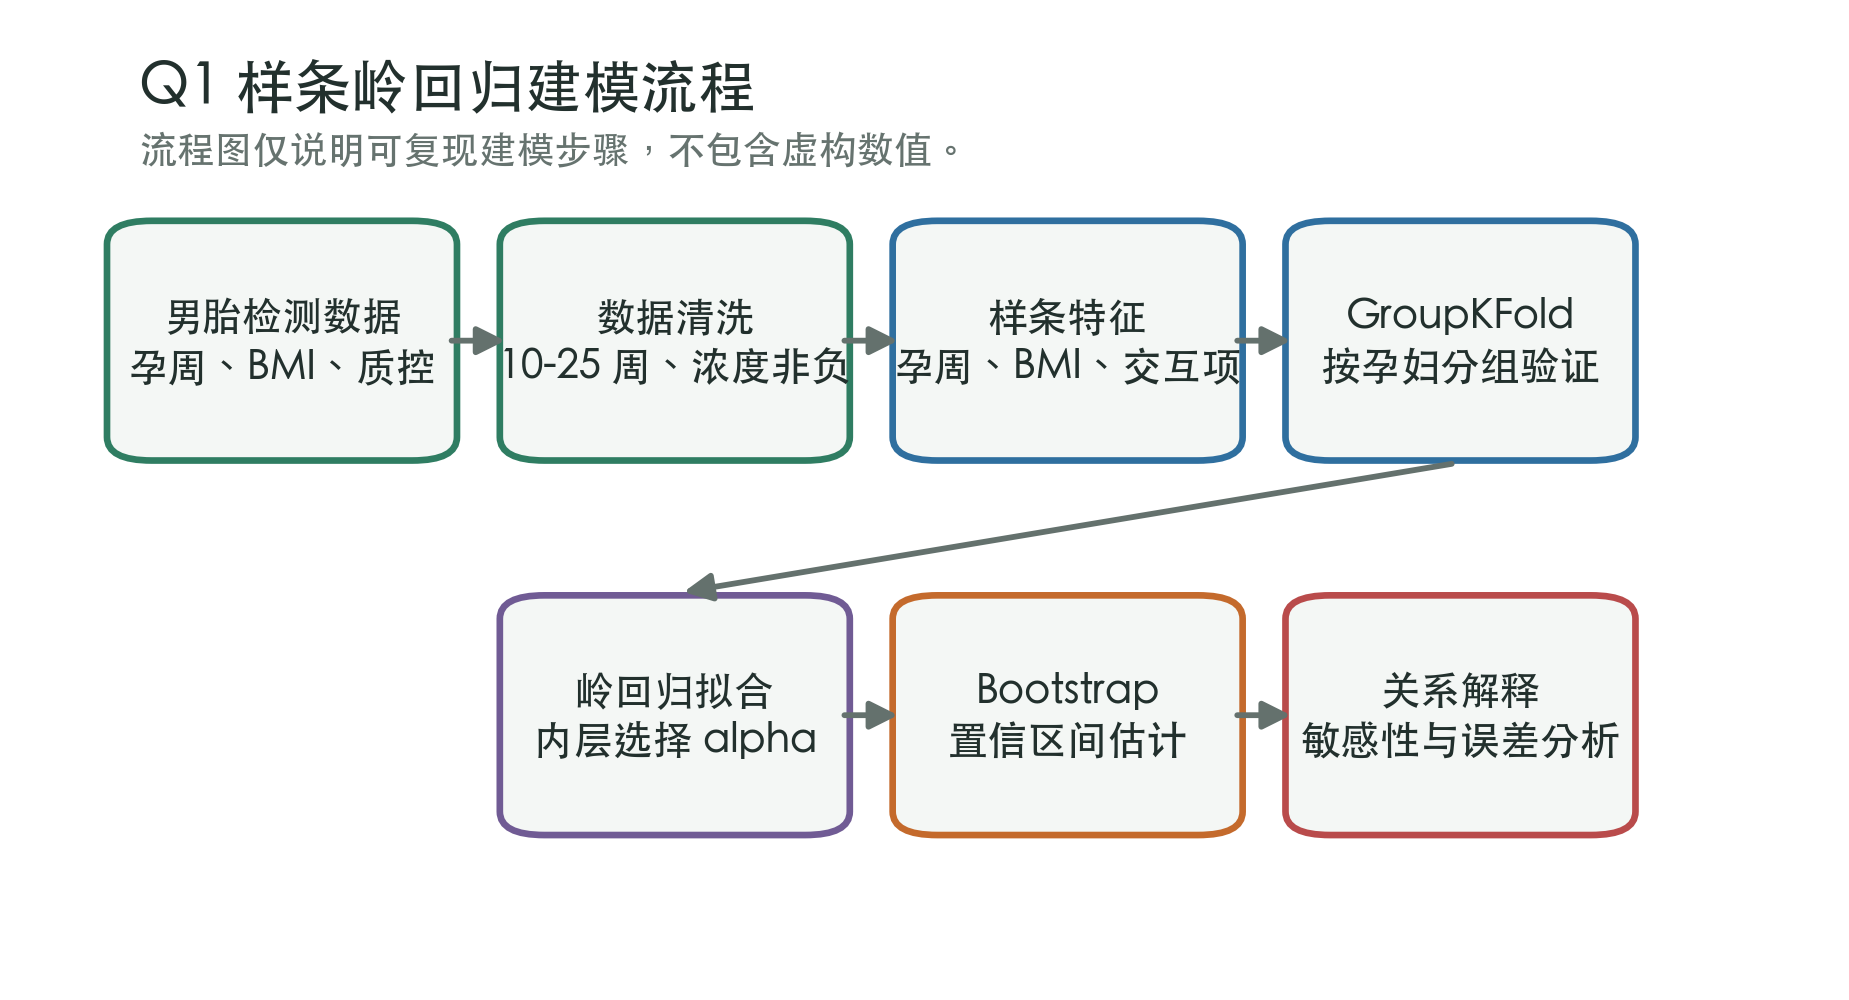
\includegraphics[width=0.76\textwidth]{figures/q1_fig5_model_flow.png}
  \caption{问题一样条岭回归建模流程}
  \label{fig:q1_flow}
\end{figure}

\subsubsection{模型结果与关系分析}

表 \ref{tab:q1_metrics} 给出了样条岭回归模型与线性基线模型的主要评价结果。样条岭回归的交叉验证 RMSE 为 0.0324，略低于线性基线的 0.0329；交叉验证 $R^2$ 为 0.0382，高于线性基线的 0.0073。这说明非线性模型相较线性基线具有一定改进，但解释度仍然有限，模型更适合用于刻画总体趋势和为后续检测时点优化提供关系基础。

\begin{table}[!ht]
  \centering
  \caption{问题一模型主要评价指标}
  \label{tab:q1_metrics}
  \begin{tabularx}{\textwidth}{cYYYY}
    \toprule
    模型 & 训练 RMSE & 训练 $R^2$ & CV-RMSE & CV-$R^2$ \\
    \midrule
    样条岭回归 & 0.0315 & 0.1208 & 0.0324 & 0.0382 \\
    线性岭回归基线 & - & - & 0.0329 & 0.0073 \\
    \bottomrule
  \end{tabularx}
\end{table}

\begin{figure}[!ht]
  \centering
  \begin{subfigure}{0.42\textwidth}
    \centering
    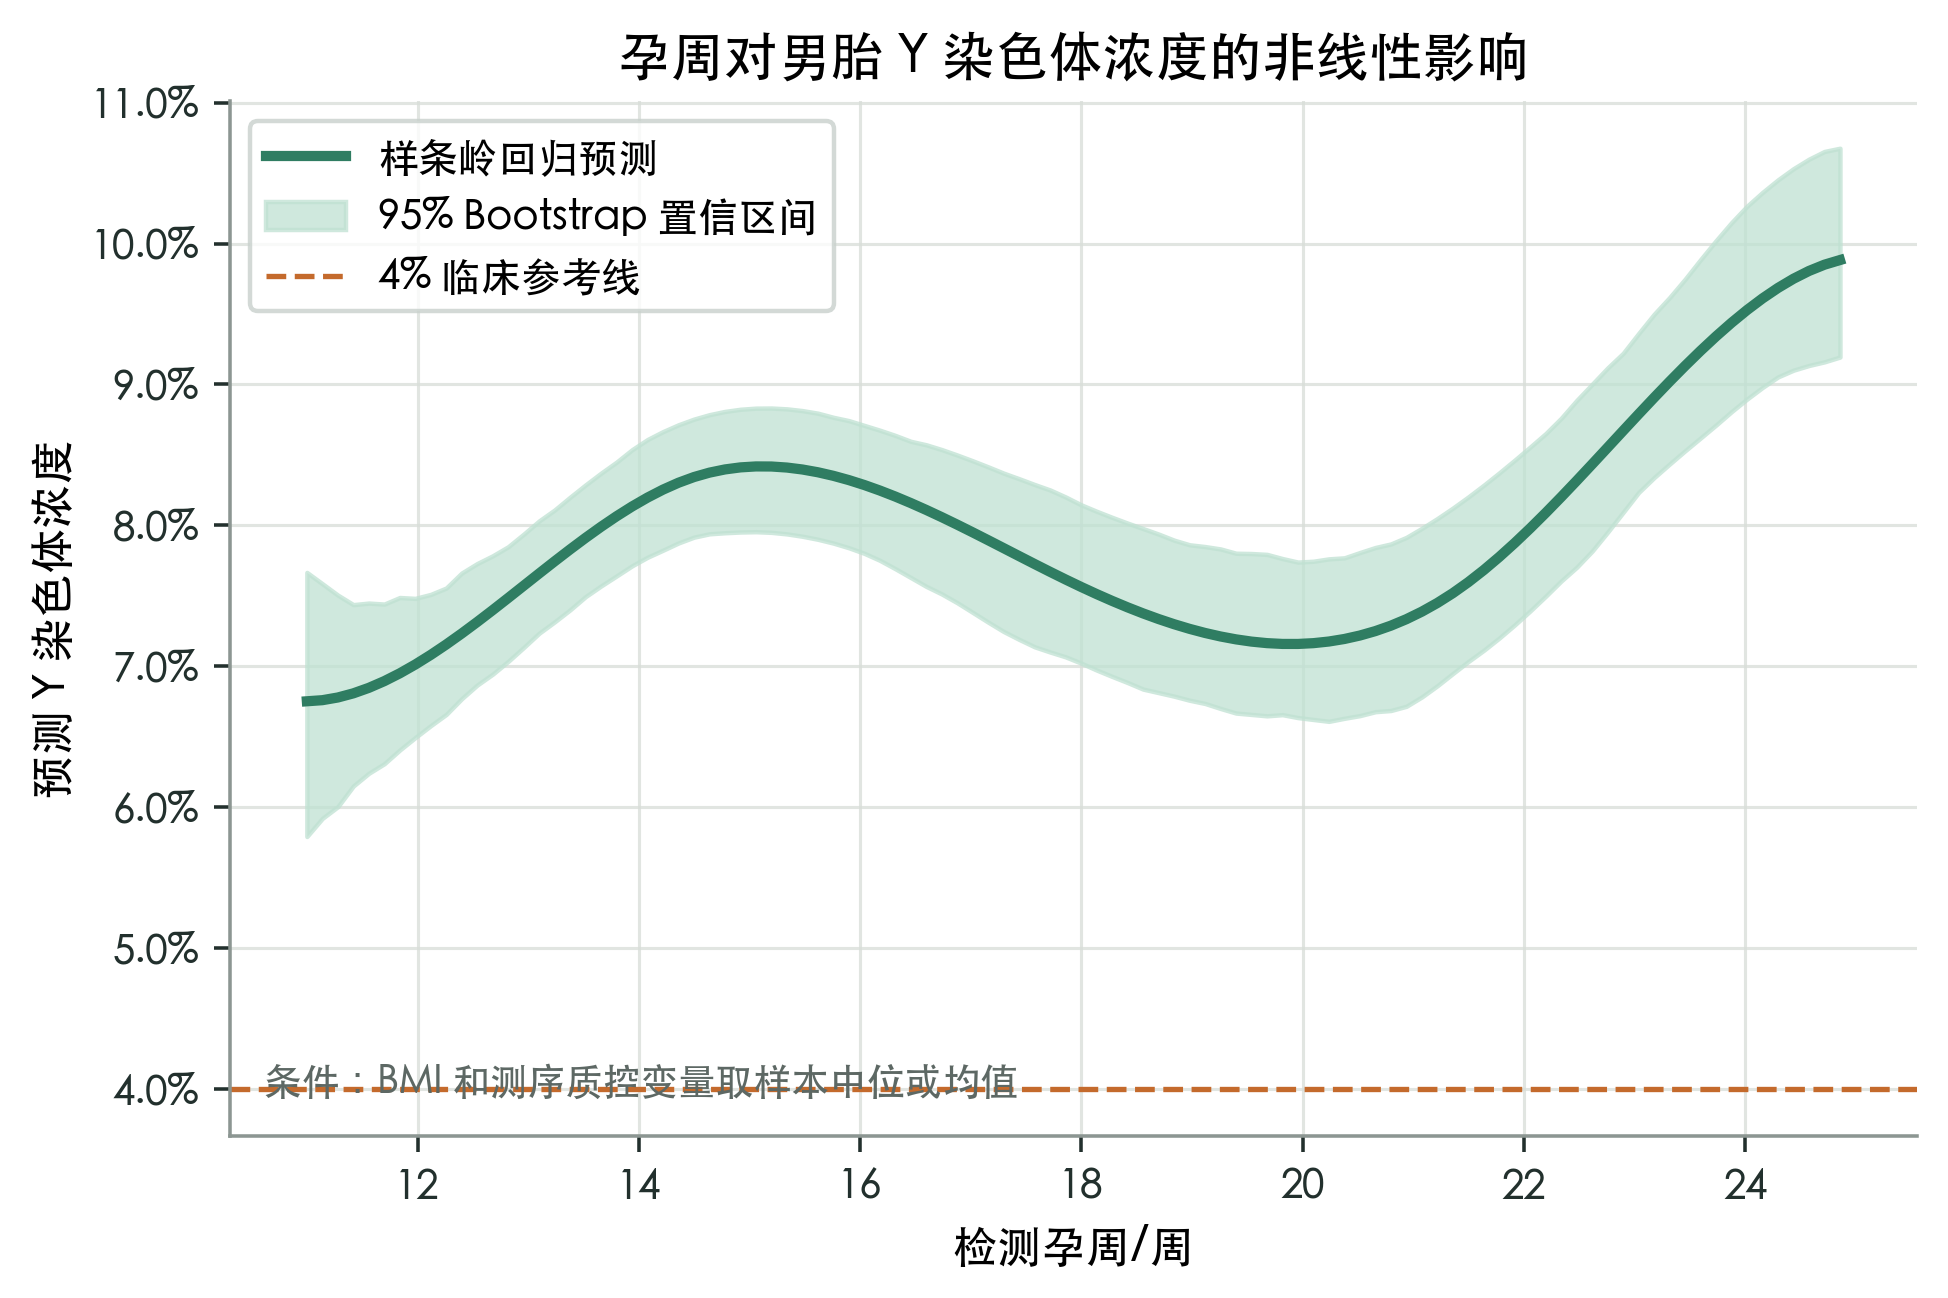
\includegraphics[width=\textwidth]{figures/q1_fig1_gestation_effect.png}
    \caption{孕周边际效应}
  \end{subfigure}
  \hspace{0.05\textwidth}
  \begin{subfigure}{0.42\textwidth}
    \centering
    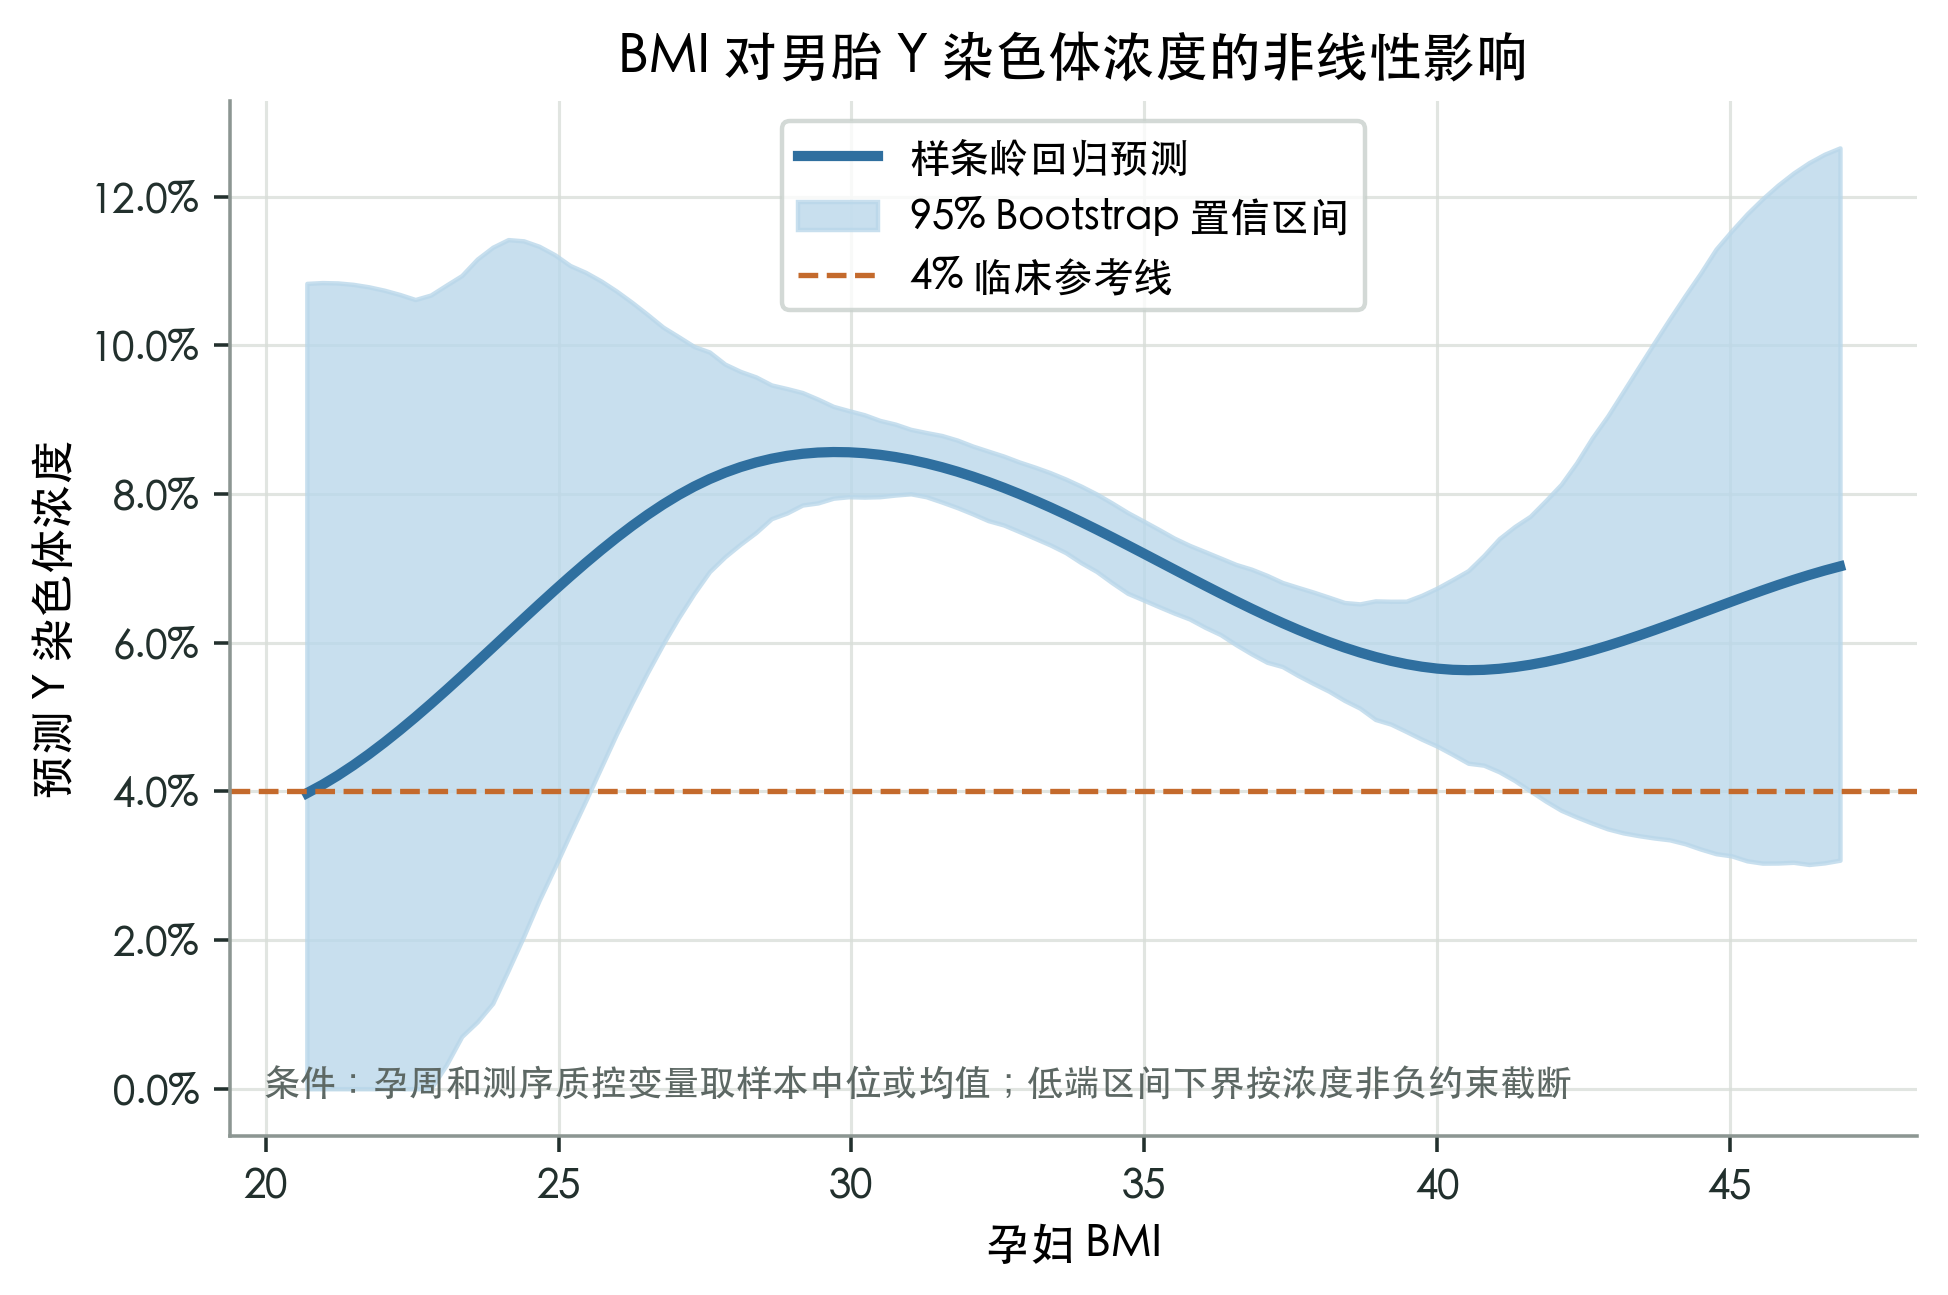
\includegraphics[width=\textwidth]{figures/q1_fig2_bmi_effect.png}
    \caption{BMI 边际效应}
  \end{subfigure}
  \caption{孕周和 BMI 对男胎 Y 染色体浓度的非线性影响}
  \label{fig:q1_effects}
\end{figure}

\FloatBarrier

从 \ref{fig:q1_effects} 可以看出，在控制 BMI 和测序质控变量后，预测的 Y 染色体浓度随孕周变化呈非线性形态：早中孕阶段有上升趋势，中间阶段略有回落，后段再次升高。BMI 的边际效应同样呈非线性，且在 BMI 边界区间置信带明显变宽，说明边界 BMI 样本支持不足，相关结论应谨慎外推。

进一步地，\ref{fig:q1_surface} 展示了孕周与 BMI 联合作用下的预测浓度面。红色曲线对应 $4\%$ 的临床参考浓度线。可以看到，在较低孕周与部分高 BMI 区域中，预测浓度接近或低于参考线；随着孕周增加，多数 BMI 区间的预测浓度上升。这一结果为第二问中根据 BMI 分组确定 NIPT 检测时点提供了直接依据。

\begin{figure}[!ht]
  \centering
  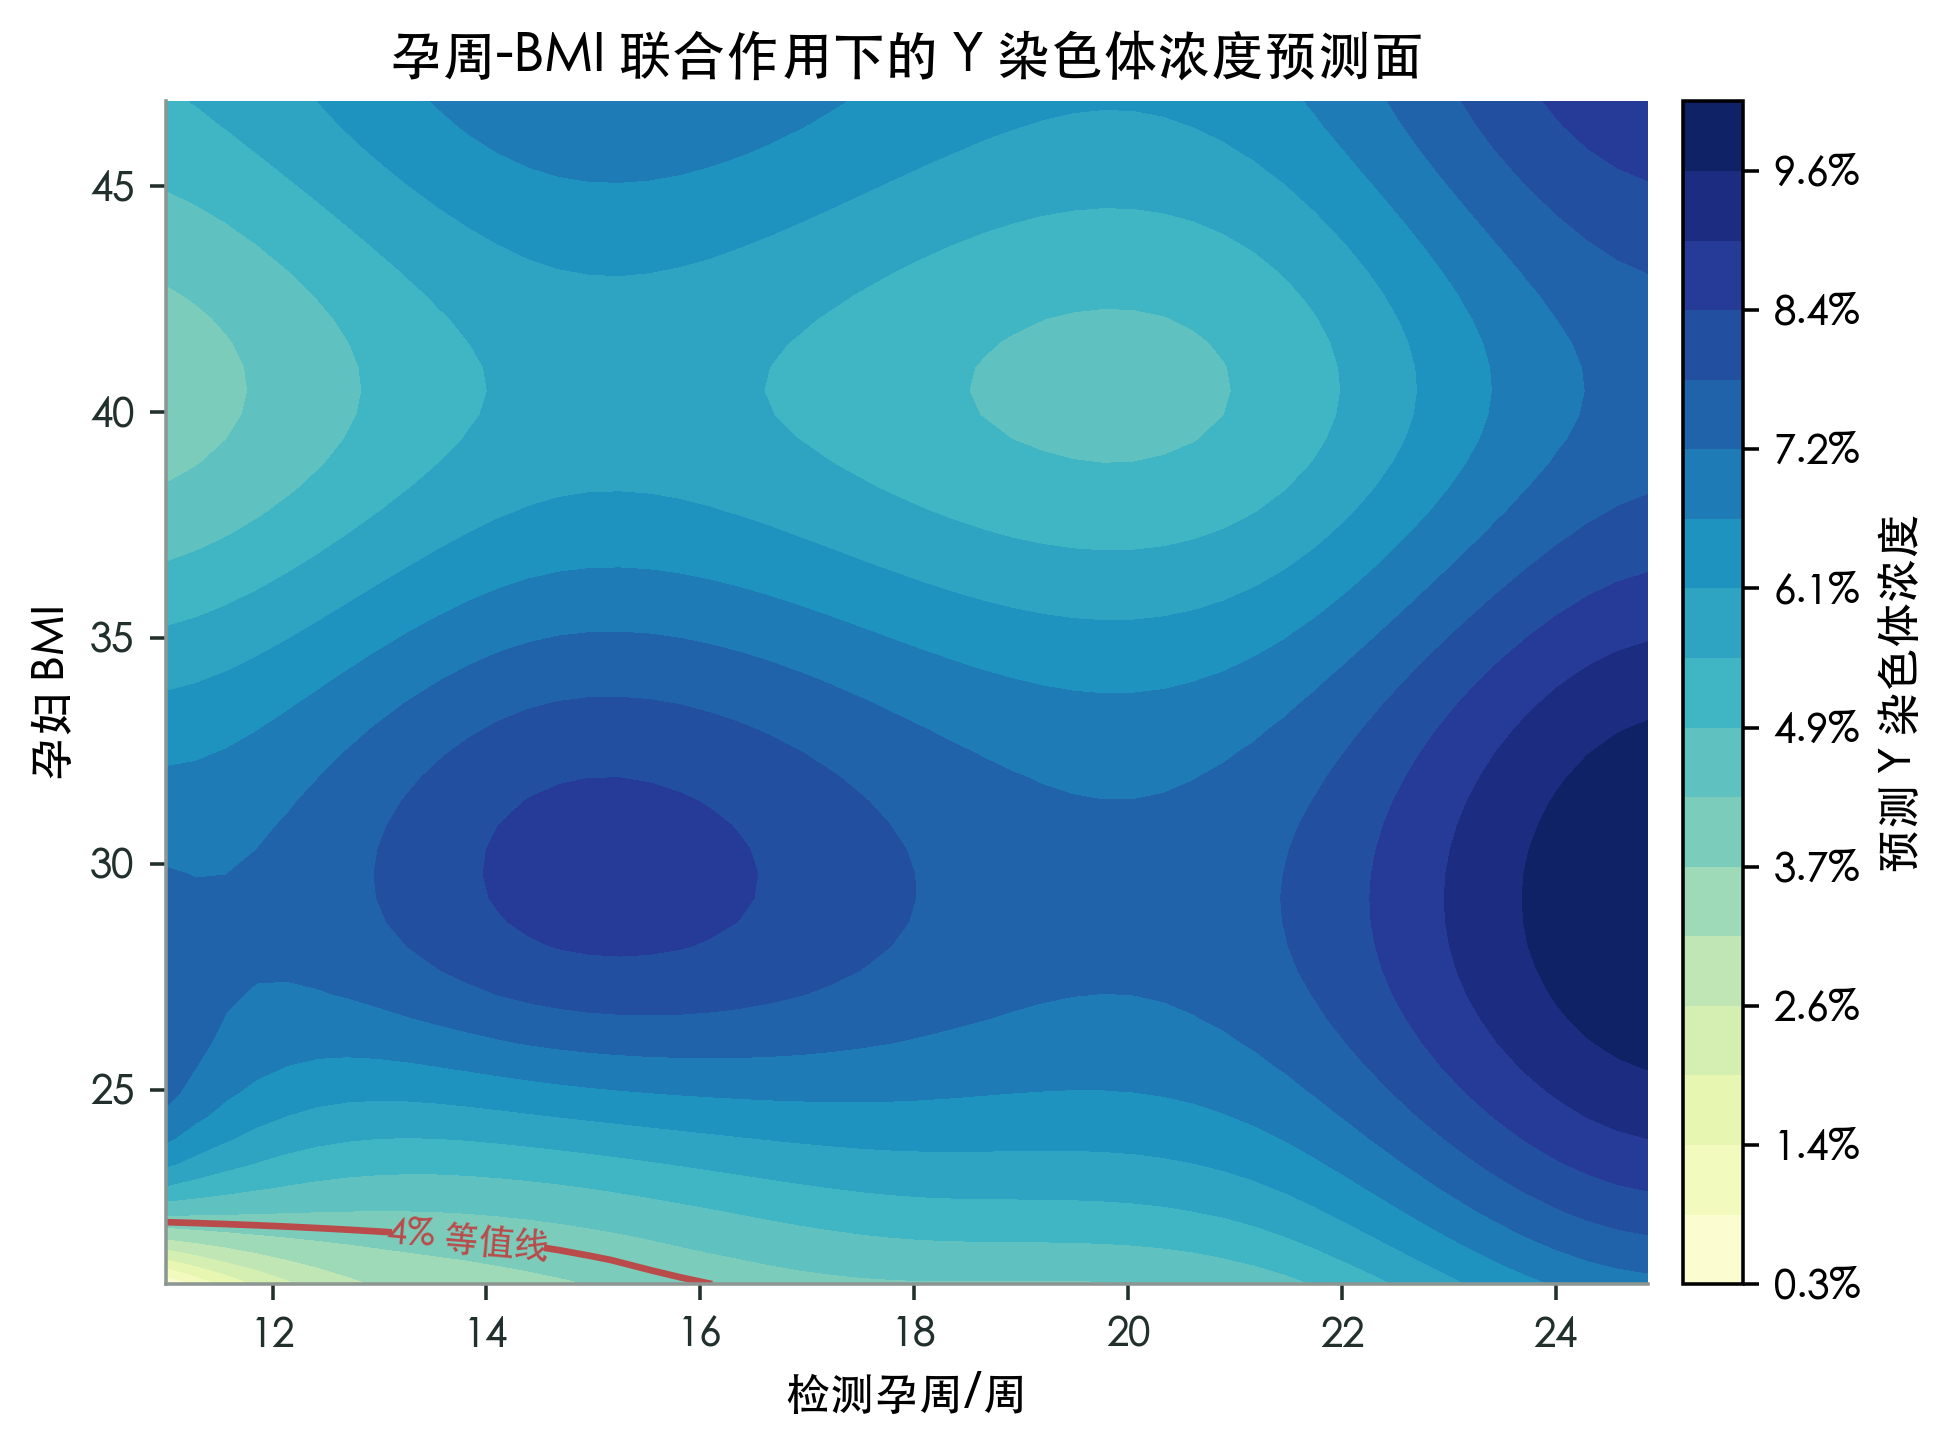
\includegraphics[width=0.56\textwidth]{figures/q1_fig3_gestation_bmi_surface.png}
  \caption{孕周和 BMI 联合作用下的 Y 染色体浓度预测面}
  \label{fig:q1_surface}
\end{figure}

\FloatBarrier

\subsubsection{敏感性与误差分析}

为检验模型稳定性，本文比较了不同样条阶数和不同孕周上界下的结果。样条阶数从 $3$ 增至 $6$ 时，CV-RMSE 的变化幅度很小，最优值出现在三阶样条；将主分析孕周上界从 $25$ 周放宽至 $26$ 周后，CV-RMSE 由 0.0324 变为 0.0324，CV-$R^2$ 由 0.0382 变为 0.0562，说明结论对孕周上界设置不敏感。

\begin{table}[htbp]
  \centering
  \caption{问题一模型检验与敏感性摘要}
  \label{tab:q1_validation}
  \begin{tabularx}{\textwidth}{cY}
    \toprule
    检验项 & 结果与解释 \\
    \midrule
    样条阶数敏感性 & 3 至 6 阶 CV-RMSE 变化幅度较小，最优阶数为 3。 \\
    孕周上界敏感性 & 上界由 25 周放宽至 26 周后，CV-RMSE 为 0.0324，结论基本稳定。 \\
    残差正态性 & Shapiro 检验 $p=5.25\mathrm{e}{-17}$，残差不满足正态假设。 \\
    残差相关性 & 残差与拟合值 Pearson $r=0.031$，$p=0.311$，未见明显线性相关。 \\
    边界不确定性 & BMI 高端样本较少，Bootstrap 原始置信区间下界曾低至 -0.0206，已按浓度非负约束截断。 \\
    \bottomrule
  \end{tabularx}
\end{table}

误差分析方面，残差 Shapiro 检验的 $p$ 值为 5.25e-17，显示残差不满足正态性假设；残差与拟合值的 Pearson 相关系数为 0.031，对应 $p$ 值为 0.311，未显示明显线性相关。BMI 边际效应的 Bootstrap 原始置信区间下界最小约为 -0.0206，按浓度非负约束截断为 $0$，反映出边界 BMI 区域预测不确定性较高。因此，后续仅将其作为趋势刻画和时点优化的关系模型，不解释为高精度医学单点预测。

\begin{figure}[htbp]
  \centering
  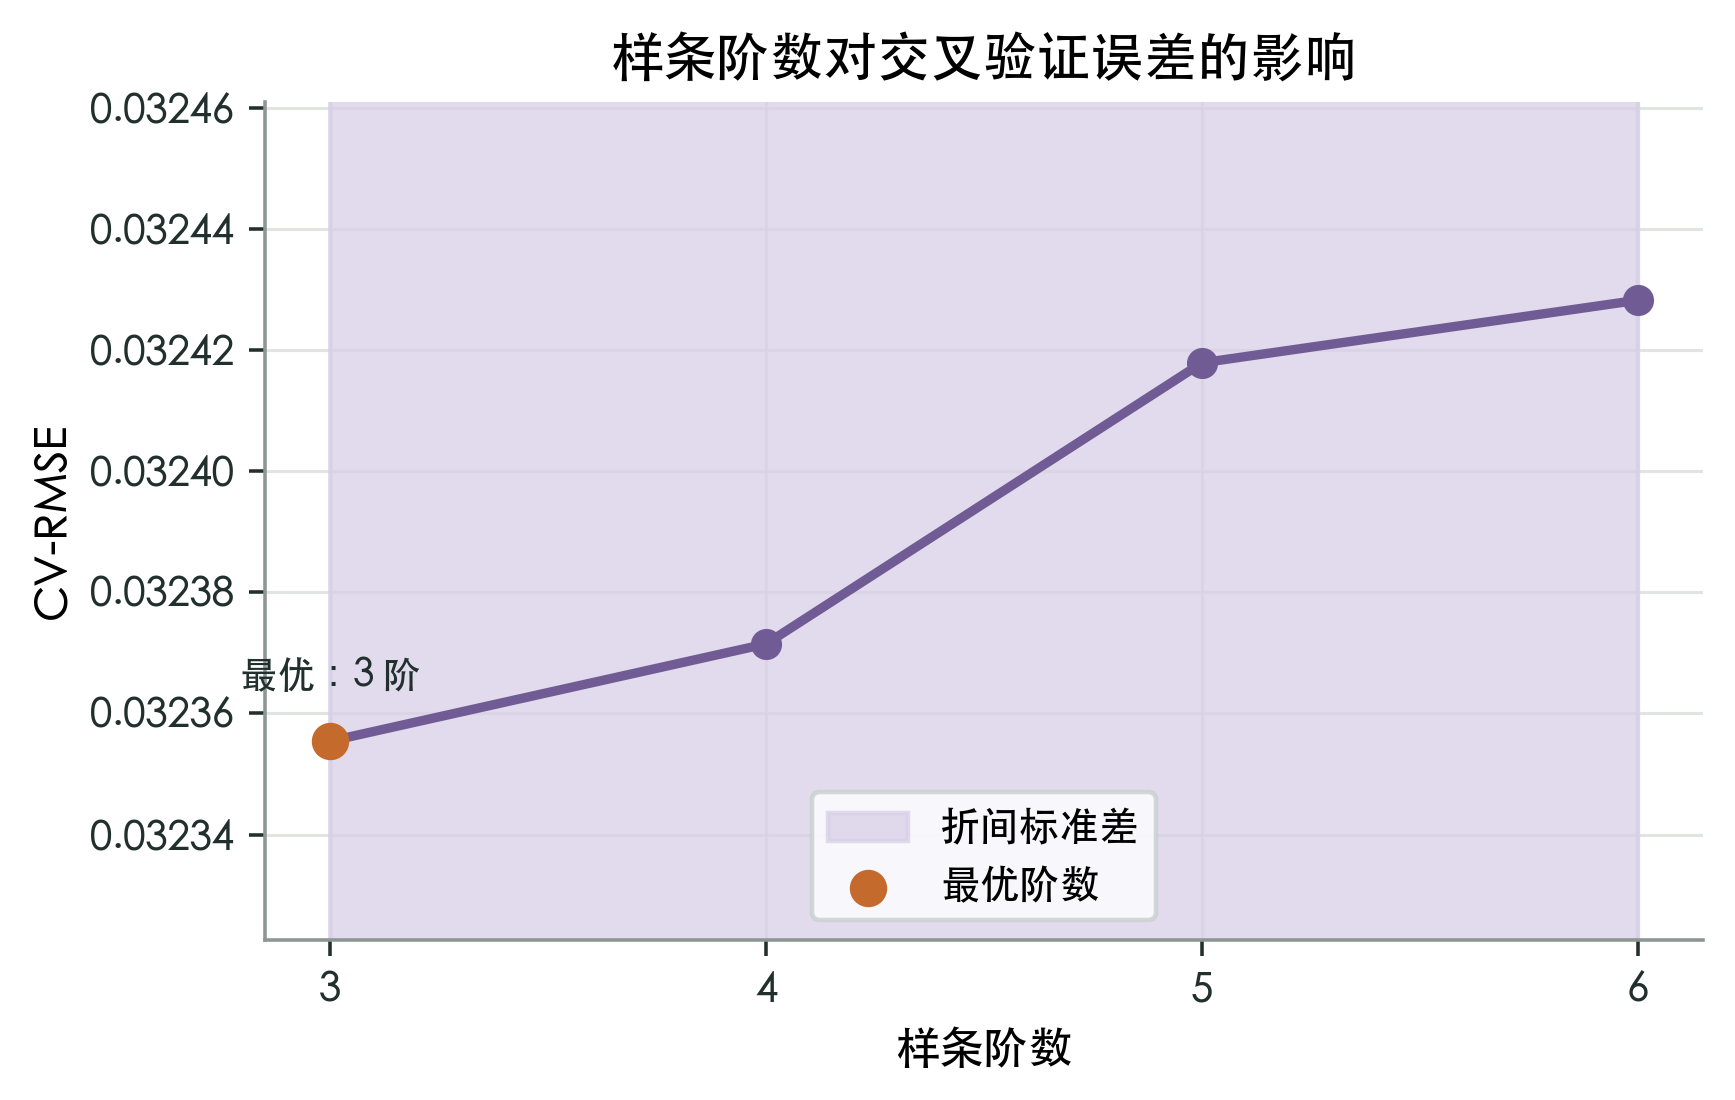
\includegraphics[width=0.66\textwidth]{figures/q1_fig4_spline_sensitivity.png}
  \caption{样条阶数对问题一交叉验证误差的影响}
  \label{fig:q1_degree_sensitivity}
\end{figure}

\FloatBarrier

\subsubsection{本问小结}

综上，问题一建立了包含孕周、BMI、二者交互项和测序质控变量的样条岭回归模型。结果表明，男胎 Y 染色体浓度与孕周、BMI 均存在非线性关系；非线性模型较线性基线有小幅稳定改进，但受个体差异和检测误差影响，整体解释度有限。后续问题将基于该模型给出的孕周-BMI 响应关系，进一步讨论 BMI 分组和最佳 NIPT 检测时点。

\subsection{问题二模型的建立与求解}\label{sub:5.2}

待用户完成方案审批和模型确认后写入。


\subsection{问题三模型的建立与求解}\label{sub:5.3}

待用户完成方案审批和模型确认后写入。


\subsection{问题4模型的建立与求解}\label{sub:5.4}

本节内容待用户完成方案审批、Claude Code 实现、Codex 复审和模型确认后写入并编译；最终中文图可在图表审批后补入。

\subsection{问题5模型的建立与求解}\label{sub:5.5}

本节内容待用户完成方案审批、Claude Code 实现、Codex 复审和模型确认后写入并编译；最终中文图可在图表审批后补入。


\section{模型的检验}\label{sec:6}
\subsection{误差分析}\label{sub:6.1}

待根据最终模型和结果补充。

\subsection{敏感性分析}\label{sub:6.2}

待根据核心参数扰动实验补充。

\subsection{鲁棒性检验}\label{sub:6.3}

待根据模型对比和数据扰动实验补充。



\section{模型的评价及推广}\label{sec:7}
\subsection{模型的优点}\label{sub:7.1}

待补充。

\subsection{模型的不足}\label{sub:7.2}

待补充。

\subsection{模型的推广}\label{sub:7.3}

待补充。



\begin{thebibliography}{99}
  \bibitem{placeholder}待补充参考文献。
\end{thebibliography}

\begin{appendixx}
  \section{源程序代码和运行说明}

本附录用于整理核心代码、运行环境和支撑材料说明。完整代码保存在支撑材料中的 \texttt{05\_code} 目录，论文附录展示关键代码片段和运行入口。

\subsection{运行环境}

\begin{itemize}
  \item 编程语言：Python，待用户确认；
  \item 主要依赖：待代码实现后补充；
  \item 运行入口：待代码实现后补充。
\end{itemize}

\subsection{核心代码}

待 Claude Code 完成代码后，由 Codex 筛选核心代码并统一附录排版。

  \section{AI 工具使用说明}

本节用于根据 \texttt{00\_shared/AI\_USAGE\_LOG.md} 整理 AI 工具使用情况。最终表述需与实际使用记录一致。

\begin{table}[htbp]
  \centering
  \caption{AI 工具使用记录摘要}
  \begin{tabularx}{\textwidth}{cYY}
    \toprule
    工具 & 用途 & 人工处理 \\
    \midrule
    Codex & 建模方案、论文草稿、图表插入和代码审查 & 待补充 \\
    Claude Code & 代码生成、运行和调试 & 待补充 \\
    \bottomrule
  \end{tabularx}
\end{table}

\end{appendixx}
\end{document}
